% INSTRUCTIONS:
% To compile this file, run "latex HW_example";  you need to do it TWICE
%    to get the cross-references (to equations, etc) to show correctly.
% Figures can be included as shown below.  If you don't have a figure,
%    comment out those lines using % signs at the beginning of each line,
%    or else just keep hitting RETURN when LaTeX gives an error message
%    saying that it can't find the figure file.
% Run "dvips HW_example.dvi" to make a Postscript file HW_example.ps,
%    and then "ps2pdf HW_example.ps" to make a PDF file HW_example.pdf.

\documentclass[12pt]{article}
\usepackage{graphicx,indentfirst}

\pagestyle{plain}
\baselineskip 18pt
\textwidth 6.5in
\textheight 7.8in
\oddsidemargin 0.1in
\evensidemargin 0.1in
\topmargin 0.3in

\newcommand{\be}{\begin{equation}}
\newcommand{\ee}{\end{equation}}
\newcommand{\reff}[1]{(\ref{#1})}


\begin{document}

\title{Computational Physics \\ Homework 5}
\author{Yi-Hsuan Hsu}
\date{11/05/2014}
\maketitle

\section{Problem}
Calculation of arbitrary testing poisson or laplace equation with Dirichlet boundary data by Gauss-Seidel algorithm. In question (c) (d), successive over-relaxation algorithm are applied and we discussing asymptotic convergence rate as function of lattice size and $w$.
\begin{equation}
		\triangle^2 \phi=f(x,y)
\end{equation}
\begin{figure}[h!]
	\begin{center}
		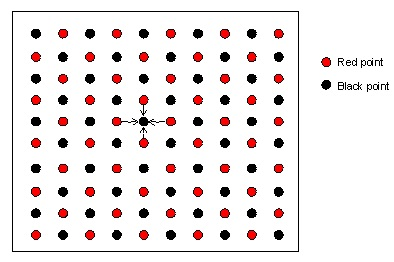
\includegraphics[width=0.8\textwidth]{redblack}
		\caption{Red-black ordering ensure guass seidel algorithm updating the new data by old data each time.}
		\label{fig1}
	\end{center}
\end{figure}


\subsection{Algorithms}
$(a)$Gauss-Seidel Algrithem with black-red ordering can be written in following equation.
\begin{eqnarray}
v_{m_1,i,j}&=&(v_{m,i-1}+v_{m,i+1,j}+v_{m,i,j-1}+v_{m,i,j+1}+h^2f_{ij})/4\\
v_{m_1,i,j}&=&(v_{m+1,i-1}+v_{m+1,i+1,j}+v_{m+1,i,j-1}+v_{m+1,i,j+1}+h^2f_{ij})/4
\end{eqnarray}
which, equation (3) is for all  nodes i,j that are red, so that we can update the red node by the old number in black node. Similarly, we update all nodes i,j that are black by the new red nodes.

$(b)$Overralaxation$(SOR)$ method optimize the successive iteration. The step of overrelaxtion on two dimensional Poission's equation with red-black ordering.
\begin{eqnarray}
v_{m_1,i,j}&=&(1-w)v_{m,i,j}+ w(v_{m,i-1}+v_{m,i+1,j}+v_{m,i,j-1}+v_{m,i,j+1}+h^2f_{ij})/4\\
v_{m_1,i,j}&=&(1-w)v_{m+1,i,j}+w(v_{m+1,i-1}+v_{m+1,i+1,j}+v_{m+1,i,j-1}+v_{m+1,i,j+1}+h^2f_{ij})/4
\end{eqnarray}
where $w=0$ is equivalent to the Gauss-Seidel method,$w<1$is underrelaxation, $w>1$is overralaxation.
(c)Convergence of Gauss-Seidel with overralaxtion parameter can be proved much faster then Jacobi and just Gauss-Seidel method. For the relaxation parameter $1<w=2/(1+sin(\frac{\pi}{N+1})<2)$ is
\begin{equation}
	\rho(R_{SOR(w)}=\frac{cos^2\frac{\pi}{N+1}}{(1+sin\frac{\pi}{N+1})}\approx1-\frac{2\pi}{N+1}
\end{equation}
which is approximately N times faster than previous method.
(d)The optimized $w$ are given below.
\begin{eqnarray}
	w_{opt}=\frac{2}{(1+\sqrt{1-\mu})^2}
\end{eqnarray}
where $\mu$ is eigenvalue of $R_{SG}$ matrix. One can proved that $\mu$ is equal to ${cos\frac{\pi}{N+1}}$,$N$ is the dimension of matrix.

Therefore, the spectral radius $\rho(R)$ can be written as
\begin{eqnarray}
&&\rho(R_{SOR(w)})= w-1, w_{opt}\leq w \leq 2\nonumber\\
&&\rho(R_{SOR(w)})= 1-w+\frac{1}{2}w^2\mu^2+w\mu\sqrt{1-w+\frac{1}{4}w^2\mu^2}, 0< w < w_{opt}\nonumber
\end{eqnarray}

\subsection{Sample output}
(a)Testing function $\phi$ and its boundary condition are defined below.
\begin{eqnarray}
&&\phi=x+xy+y+1\nonumber\\
&&\phi_{xx}+\phi_{yy}=0\nonumber\\
&&\phi(x,y)=0\ ,\ at\ all\ boundary
\end{eqnarray}
Figure(2) are the result of convergence rate,$N=8,16,32$, versus relaxation parameter, the behavior of experimental convergence rate fit theory better in small $N$ than large $N$. In $N=16$, some displacement are exist near and after $w_{opt}$. At the same time, experimental curve are lower than theory at $w~1$ in picture of $N=16$, and points after $w_{opt}$ become more sparse. 

\begin{figure}[h!]
	\begin{center}
		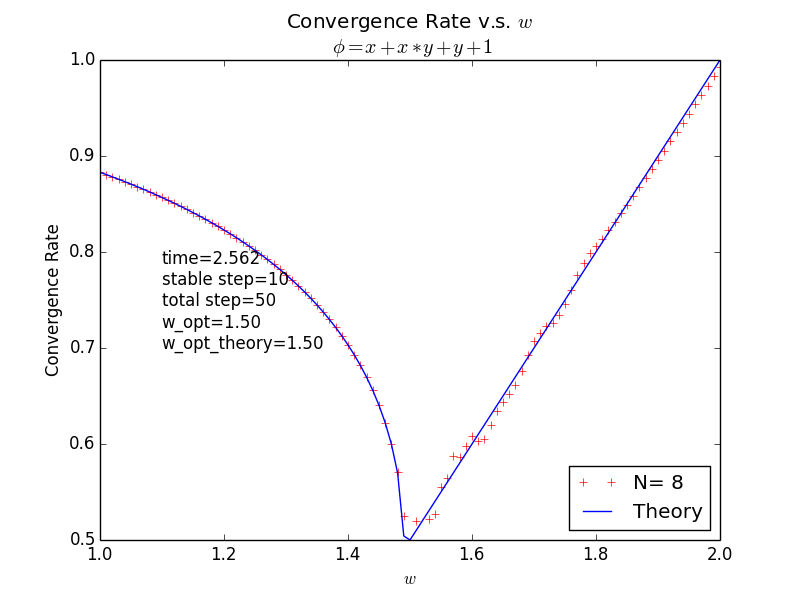
\includegraphics[width=0.4\textwidth]{Conv_rate_N_8.png}
		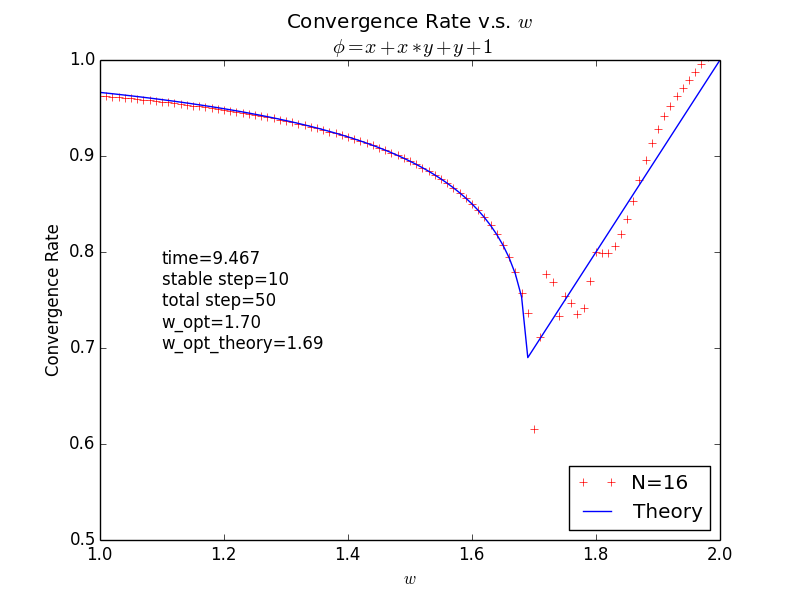
\includegraphics[width=0.4\textwidth]{Conv_rate_N_16.png}
		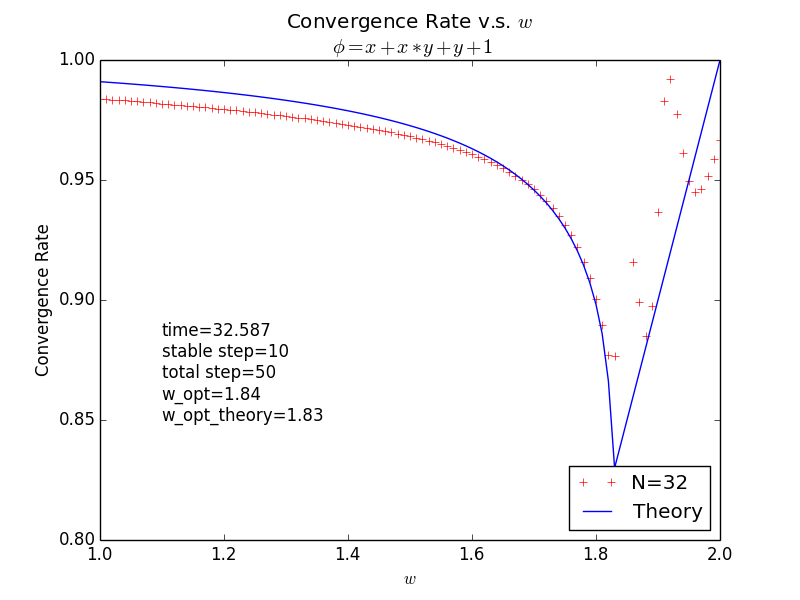
\includegraphics[width=0.4\textwidth]{Conv_rate_N_32.png}
		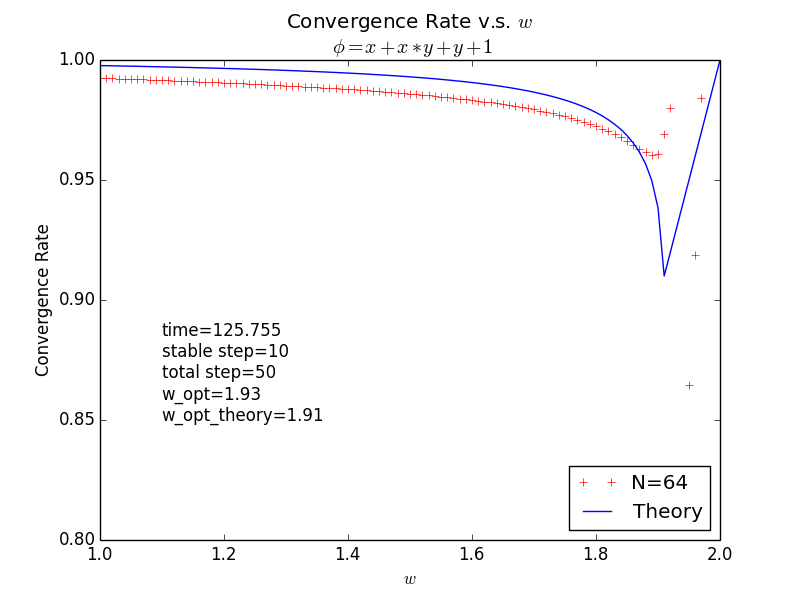
\includegraphics[width=0.4\textwidth]{Conv_rate_N_64.png}
		\caption{Convergence rate versus relaxation parameter. Lower text shows the operating time, warm up step, and total step. Optimal w in experiment and theory are fund to be close.}
		\label{fig2}
	\end{center}
\end{figure}
The second function taken into the test is
\begin{eqnarray}
&&\phi=x^3+y^3\nonumber\\
&&\phi_{xx}+\phi_{yy}=6(x+y)\nonumber\\
&&\phi(0,y)=y^3\nonumber\\
&&\phi(1,y)=y^3+1\nonumber\\
&&\phi(x,0)=x^3\nonumber\\
&&\phi(x,1)=x^3+1
\end{eqnarray} 

\begin{figure}[h!]
	\begin{center}
		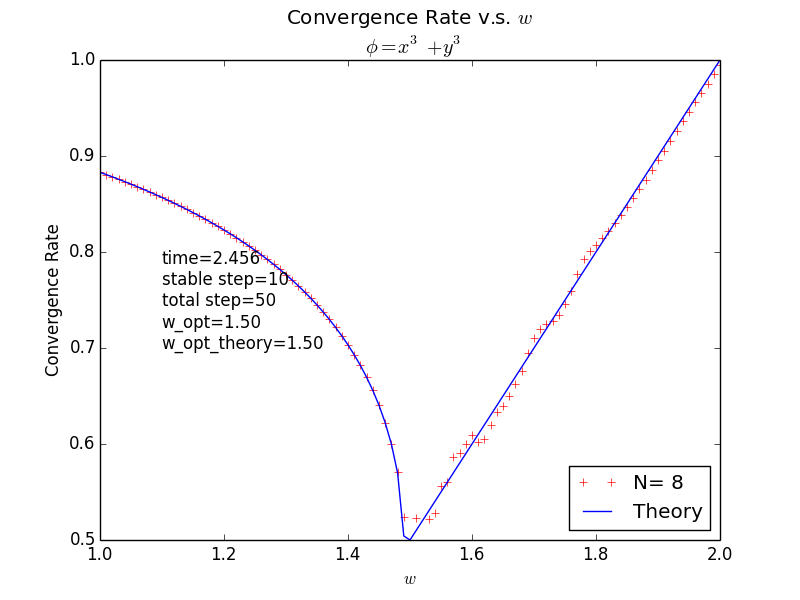
\includegraphics[width=0.4\textwidth]{Conv_rate_N_8_2.png}
		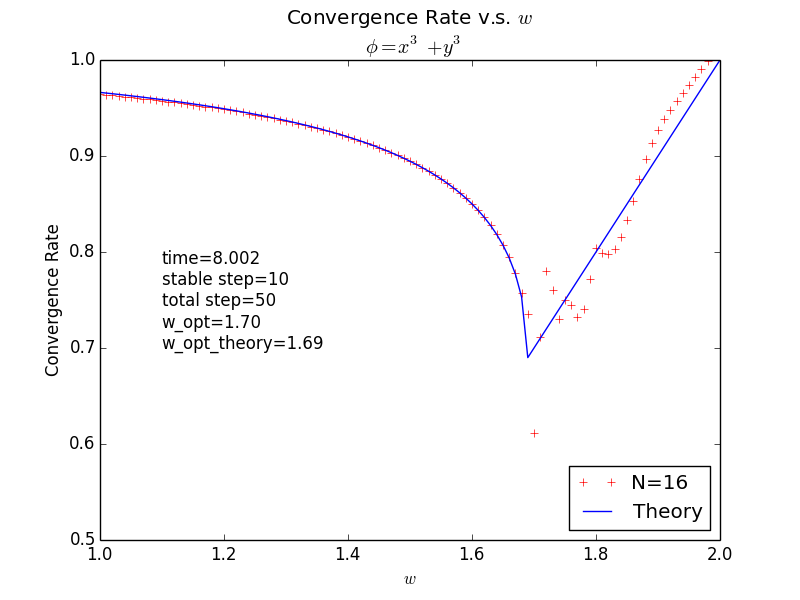
\includegraphics[width=0.4\textwidth]{Conv_rate_N_16_2.png}
		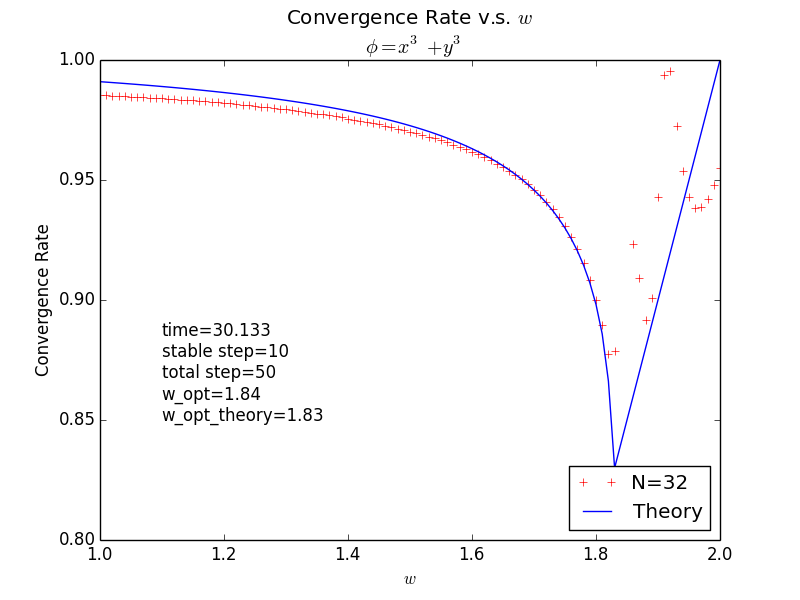
\includegraphics[width=0.4\textwidth]{Conv_rate_N_32_2.png}
		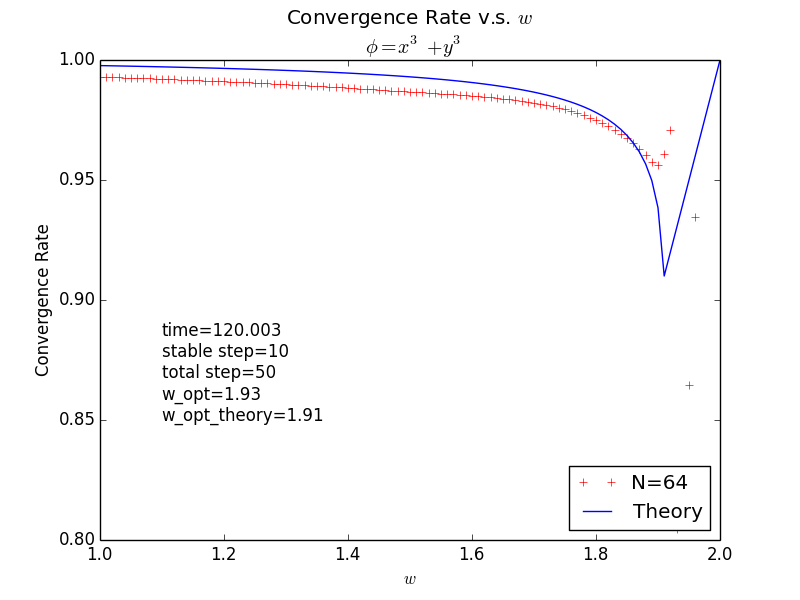
\includegraphics[width=0.4\textwidth]{Conv_rate_N_64_2.png}
		\caption{Convergence rate versus relaxation parameter. Lower text shows the operating time, warm up step, and total step. Optimal w in experiment and theory are fund to be close. Compare to different testing function we can conclude that the behavior of convergence rate is independent of solution, boundary condition but depends on lattice size.}
		\label{fig3}
	\end{center}
\end{figure}

We can observe the same behavior as well as in the previous pictures. As a result, one can conclude that the asymptotic convergence rate are independence of particular function, boundary data or initial guess.

\begin{figure}[h!]
	\begin{center}
		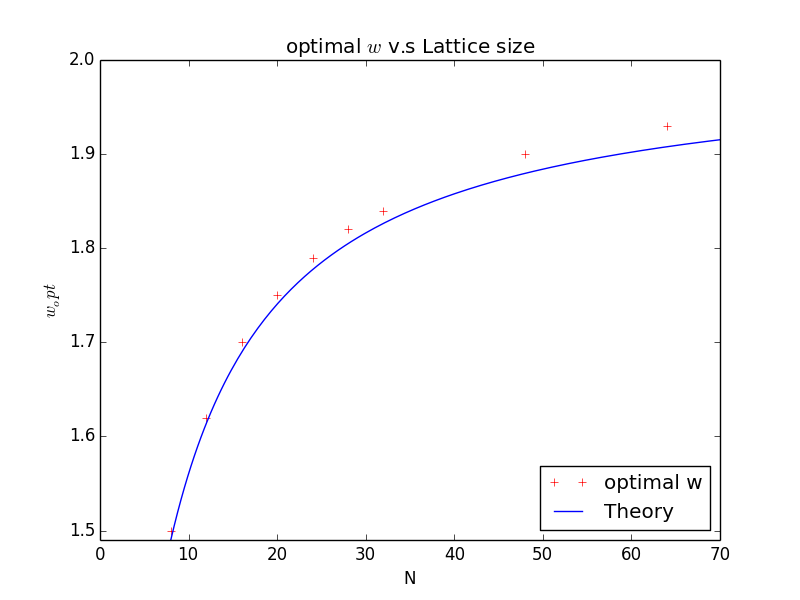
\includegraphics[width=0.4\textwidth]{optimal.png}
		\caption{The convergence rate versus relaxation parameter.}
		\label{fig4}
	\end{center}
\end{figure}
Figure 4 picture the optimal w v.s. lattice size. Compare the experiment and theory, experiment fit theory well when N is small. When N goes up, optimal w from experiment become larger than predict.

\begin{figure}[h!]
	\begin{center}
		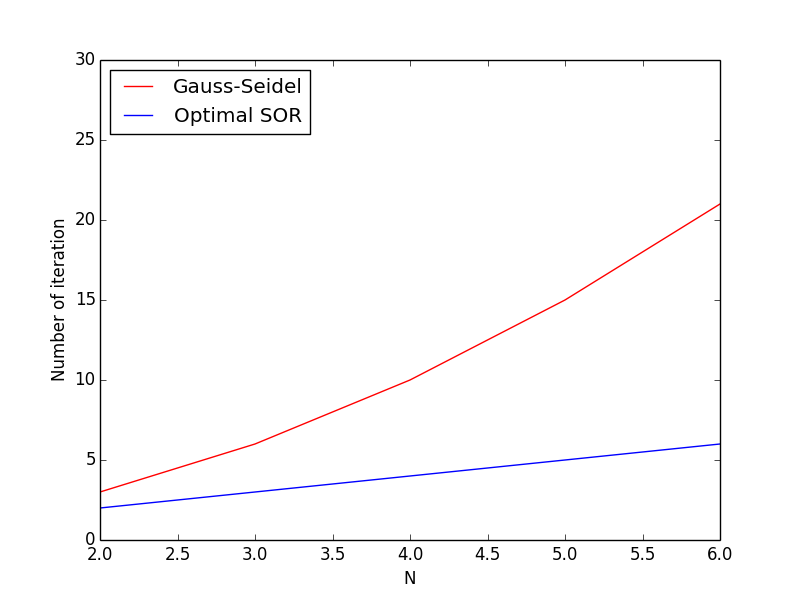
\includegraphics[width=0.4\textwidth]{iteraion.png}
		\caption{Number of iteration to reduce error by 100 time than initial guess.}
	\end{center}
\end{figure}
Figure 5 illustrated that the number of iteration to reduce error by optimal w grows much slower than GS method do. 


\end{document}



\begin{figure}[h!]
	\begin{center}
		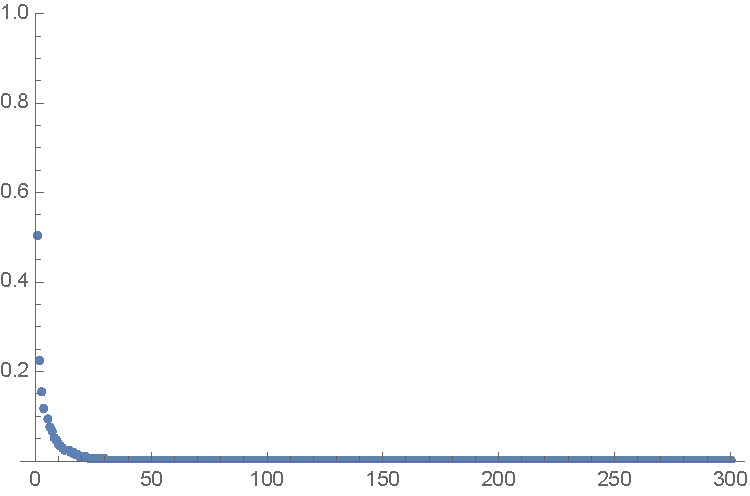
\includegraphics[width=0.4\textwidth]{a_09.pdf}
		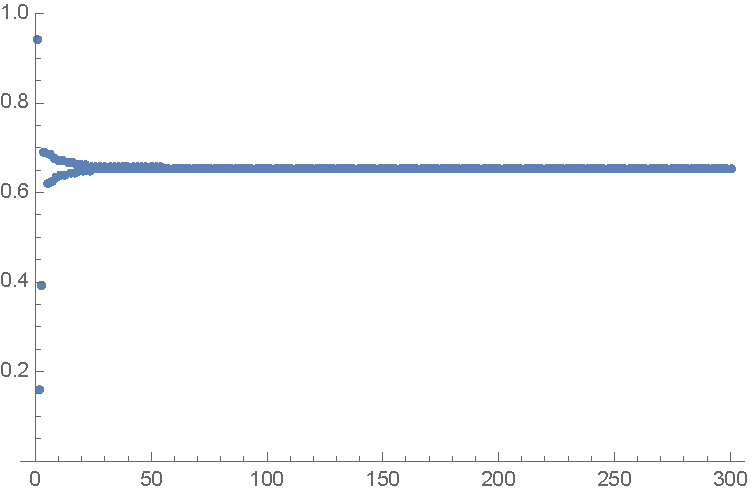
\includegraphics[width=0.4\textwidth]{a_29.pdf}
		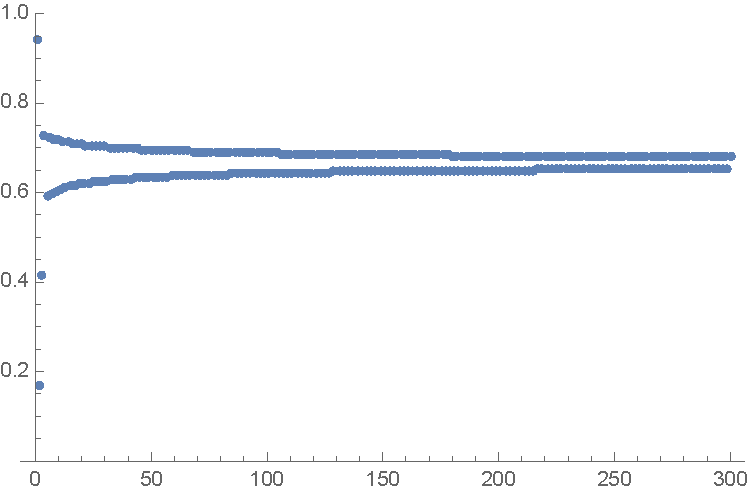
\includegraphics[width=0.4\textwidth]{a_30.pdf}
		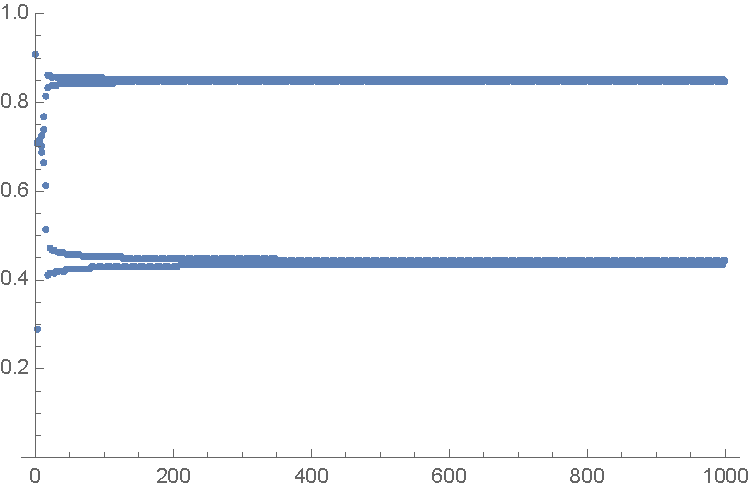
\includegraphics[width=0.4\textwidth]{a_3449.pdf}
		\caption{logistic map. Upper, left a=0.99, right a=2.9. Lower, left a=3.0, right a=3.4494.}
	\end{center}
\end{figure}

\begin{figure}[b!]
	\begin{center}
		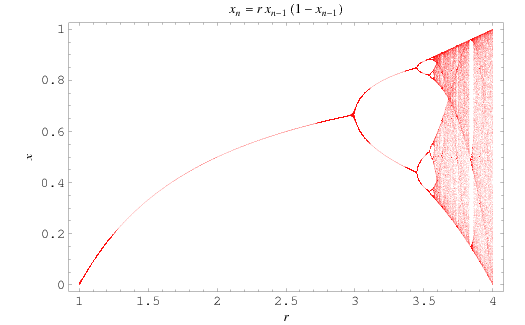
\includegraphics[width=0.8\textwidth]{logistic_map.png}
		\caption{bifurcation diagram of the logistic map. Pic. from Mahtworld}
		\label{fig1}
	\end{center}
\end{figure}


\begin{table}[h!]
	\begin{tabular}{c|lr}
		\hline
		A & $Table$ & Is\\ 
		Messy & To & Write\\
		\hline
	\end{tabular}
\end{table}


\begin{table}[h]
	\begin{center}
		\begin{tabular}{c|c}
			\hline
			period & bifurcation point a\\ 
			\hline
			2 & $0.7199616841972$ \\
			4 & $0.8332663532346$\\
			8 & $0.8591690091416$\\
			16& $0.8640801075000$*\\
			\hline
		\end{tabular}
	\end{center}
	\caption{Numerical approach to recursion sin function. First three are searching by bisection method, $\epsilon<10^{-10}$. *Last one is using step-in method, accuracy$\epsilon<10^{-5}$, although steps are much smaller than that.}
\end{table}

\begin{eqnarray}
G&&=6.67\times 10^{11} m^3 kg^{-1} s^{-2}\nonumber\\
M_{sun}&&=1.988\times 10^{30} kg\nonumber\\
c&&=3.0\times 10^8 ms^{-1}\nonumber\\
R_{orbit}&&=46\times 10^9 m\nonumber\\
v&&=58.98\times 10^3 ms^{-1}\nonumber\\
T_{period}&&=87.968 days
\end{eqnarray}